\chapter{検証・評価}
本章では提案したDNA配列アラインメントスコア計算用の光Race Logic回路について機能検証と評価を行う.
\section{検証}
検証に用いたのはOptiwave社が提供するOptisystemというシミュレータである.
OptiSystemは光ネットワークのあらゆるタイプの広範囲のシステムの設計,評価,シミュレーションを行なうソフトウェアである.
素子レベルからシステムレベルまでの物理レイヤー上の光通信システムの設計と解析を行うことができる.

配列長N=2のアラインメントスコアを求める提案回路について,光Race Logic arrayの動作を確認した.
今回のシミュレーションにおいて,各素子において光伝搬信号に影響を与える雑音や損失は考慮していない.
またOptisystemの仕様上,遅延素子で付与された遅延時間のみが考慮され,
素子や導波路の伝搬遅延については考慮されていない.
検証するスイッチの状態を図\ref{fig:test_swich}に,
シミュレーションの結果を図\ref{fig:test}に示す.
\begin{figure}[t!]
\begin{center}
\subfigure[配列が完全一致のスイッチ状態]{
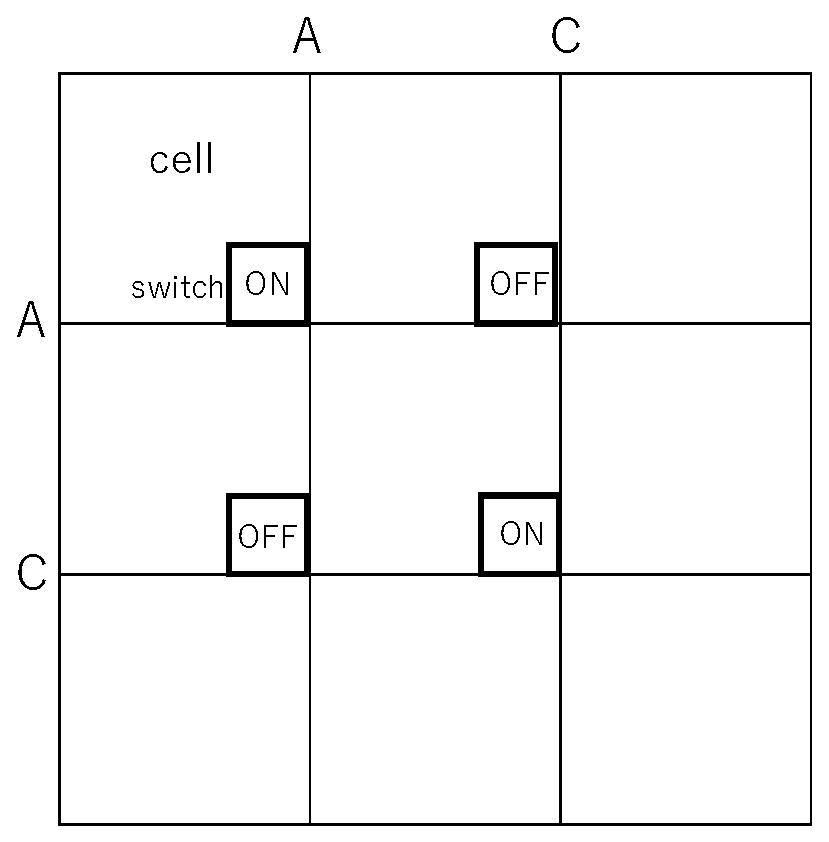
\includegraphics[keepaspectratio,scale=0.3]{fig/4/test_swich_a.eps}
\label{fig:test_swich_a}}
\subfigure[配列が一部一致の場合のスイッチ状態]{
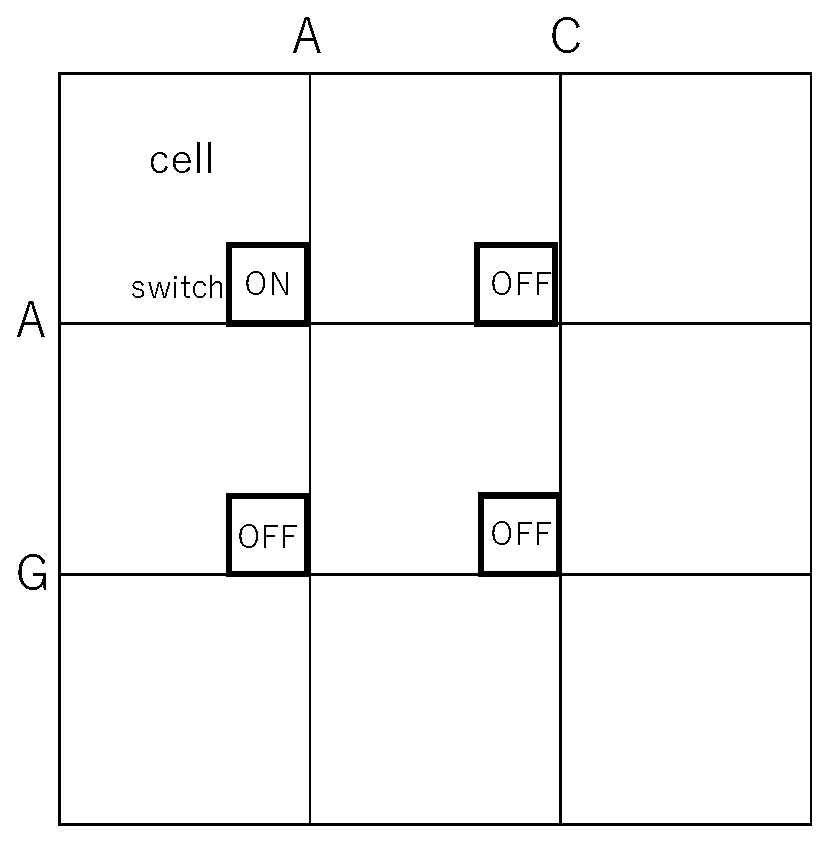
\includegraphics[keepaspectratio,scale=0.3]{fig/4/test_swich_b.eps}
\label{fig:test_swich_b}}
\subfigure[配列が完全不一致の場合のスイッチ状態]{
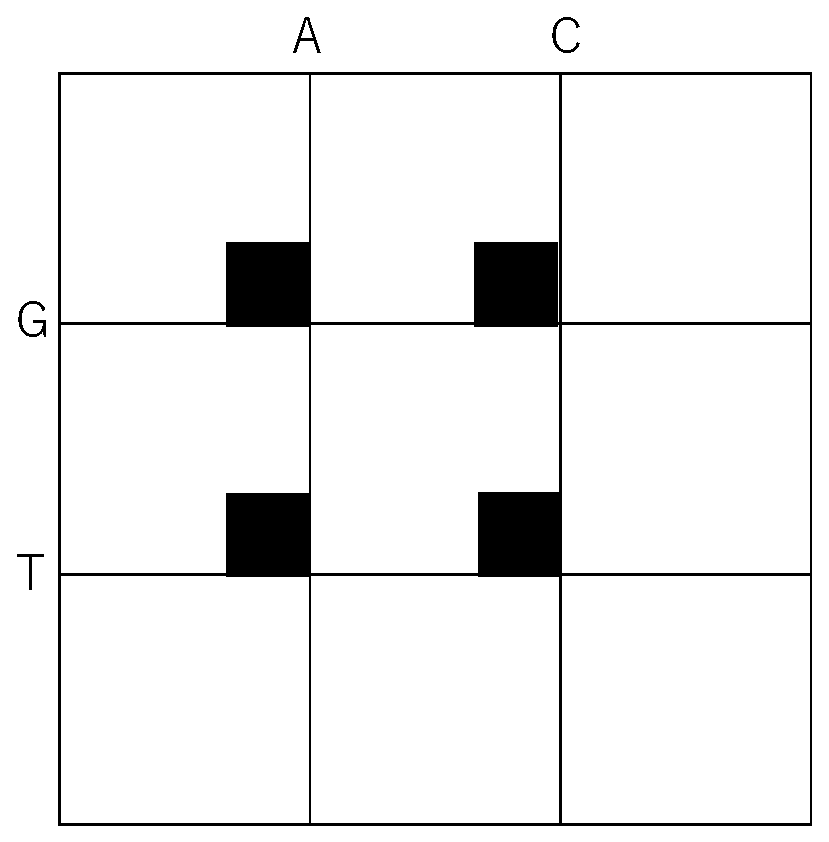
\includegraphics[keepaspectratio,scale=0.3]{fig/4/test_swich_c.eps}
\label{fig:test_swich_c}}
\caption{配列長N=2における光Race Logic arrayのスイッチ状態}
\label{fig:test_swich}
\end{center}
\end{figure}
\begin{figure}[t!]
\begin{center}
\subfigure[光Race Logic arrayへの光伝搬入力信号強度]{
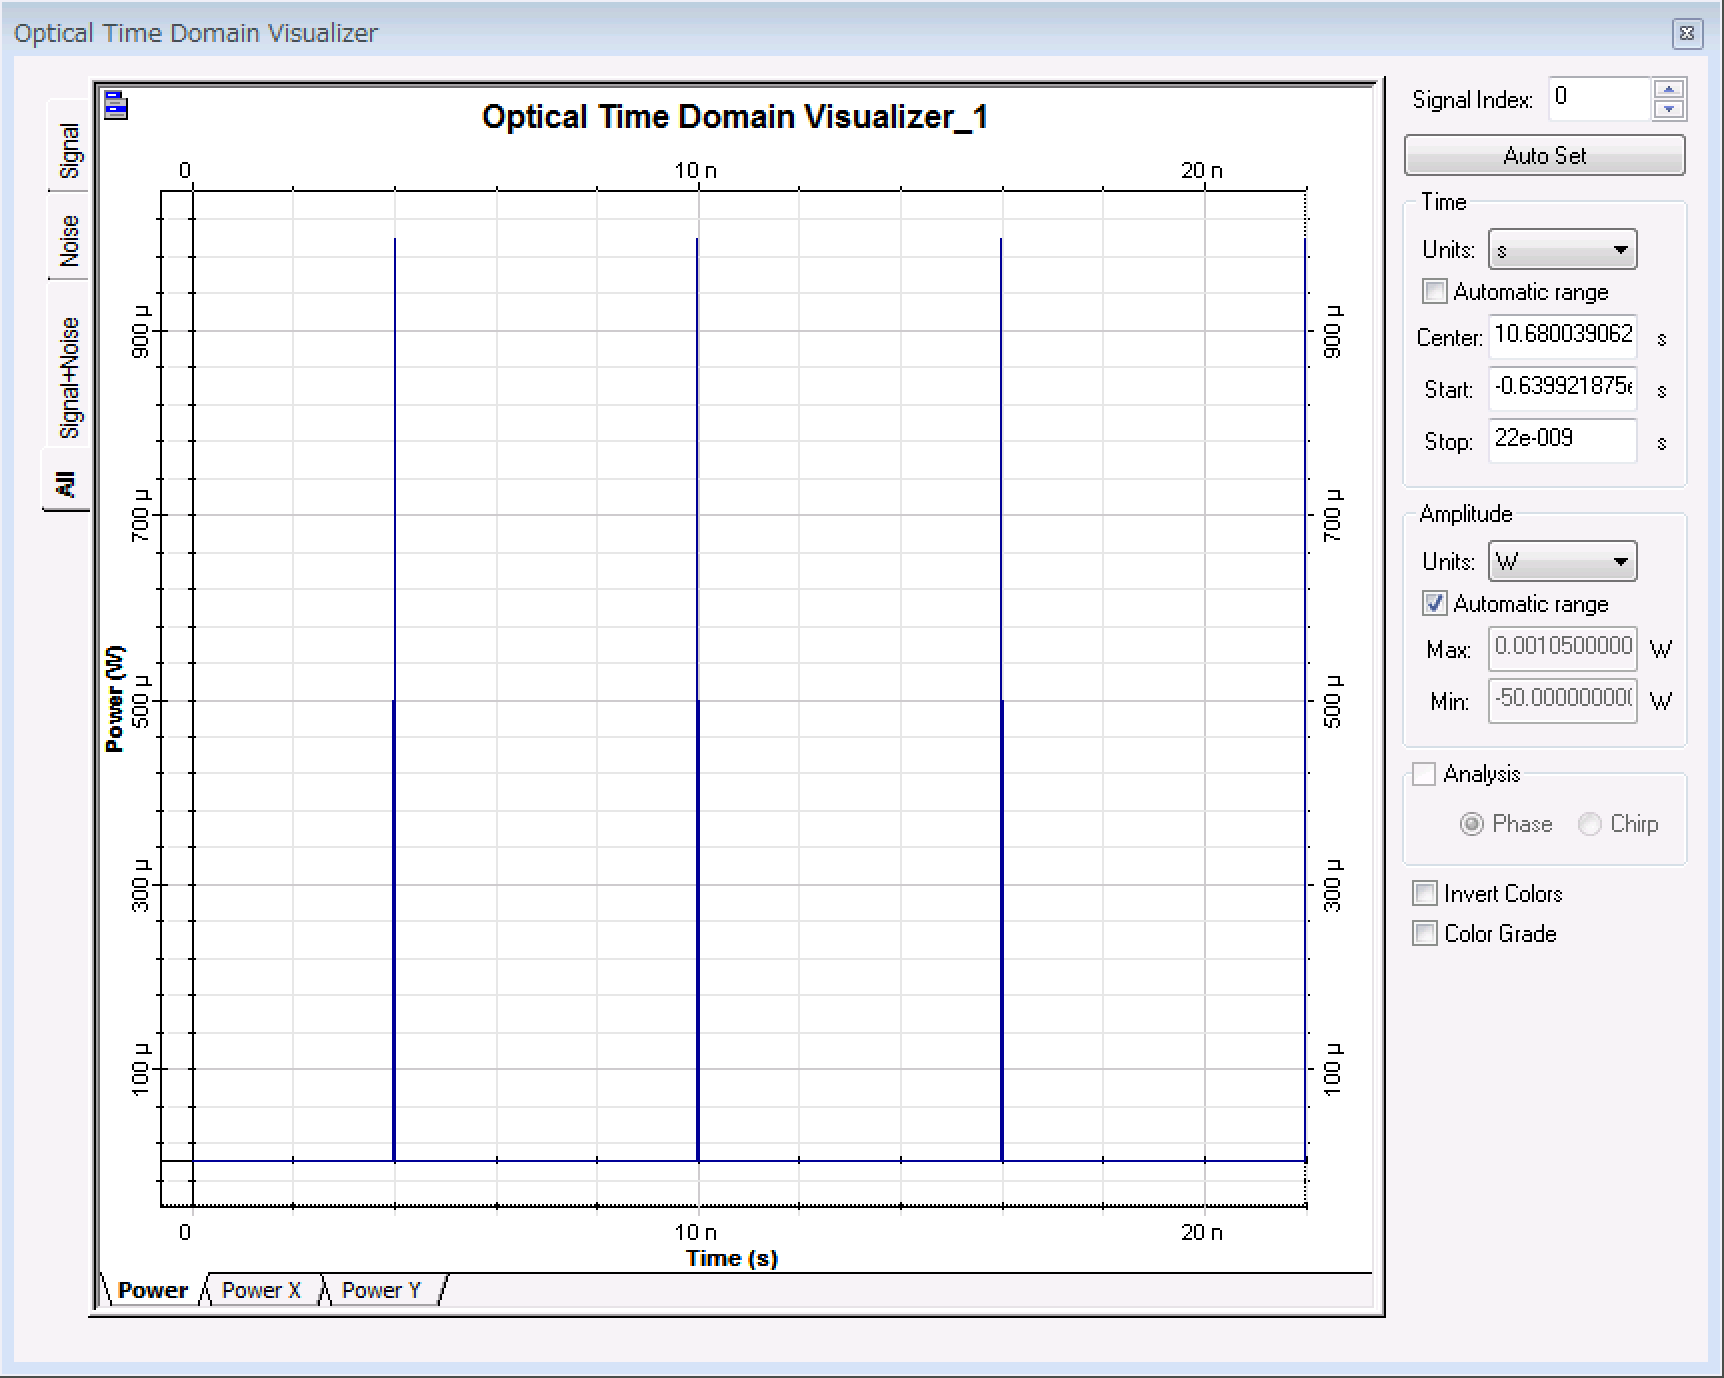
\includegraphics[keepaspectratio,scale=0.5]{fig/4/test_in.png}
\label{fig:test_in}}
\subfigure[光Race Logic arrayへの光伝搬出力信号強度]{
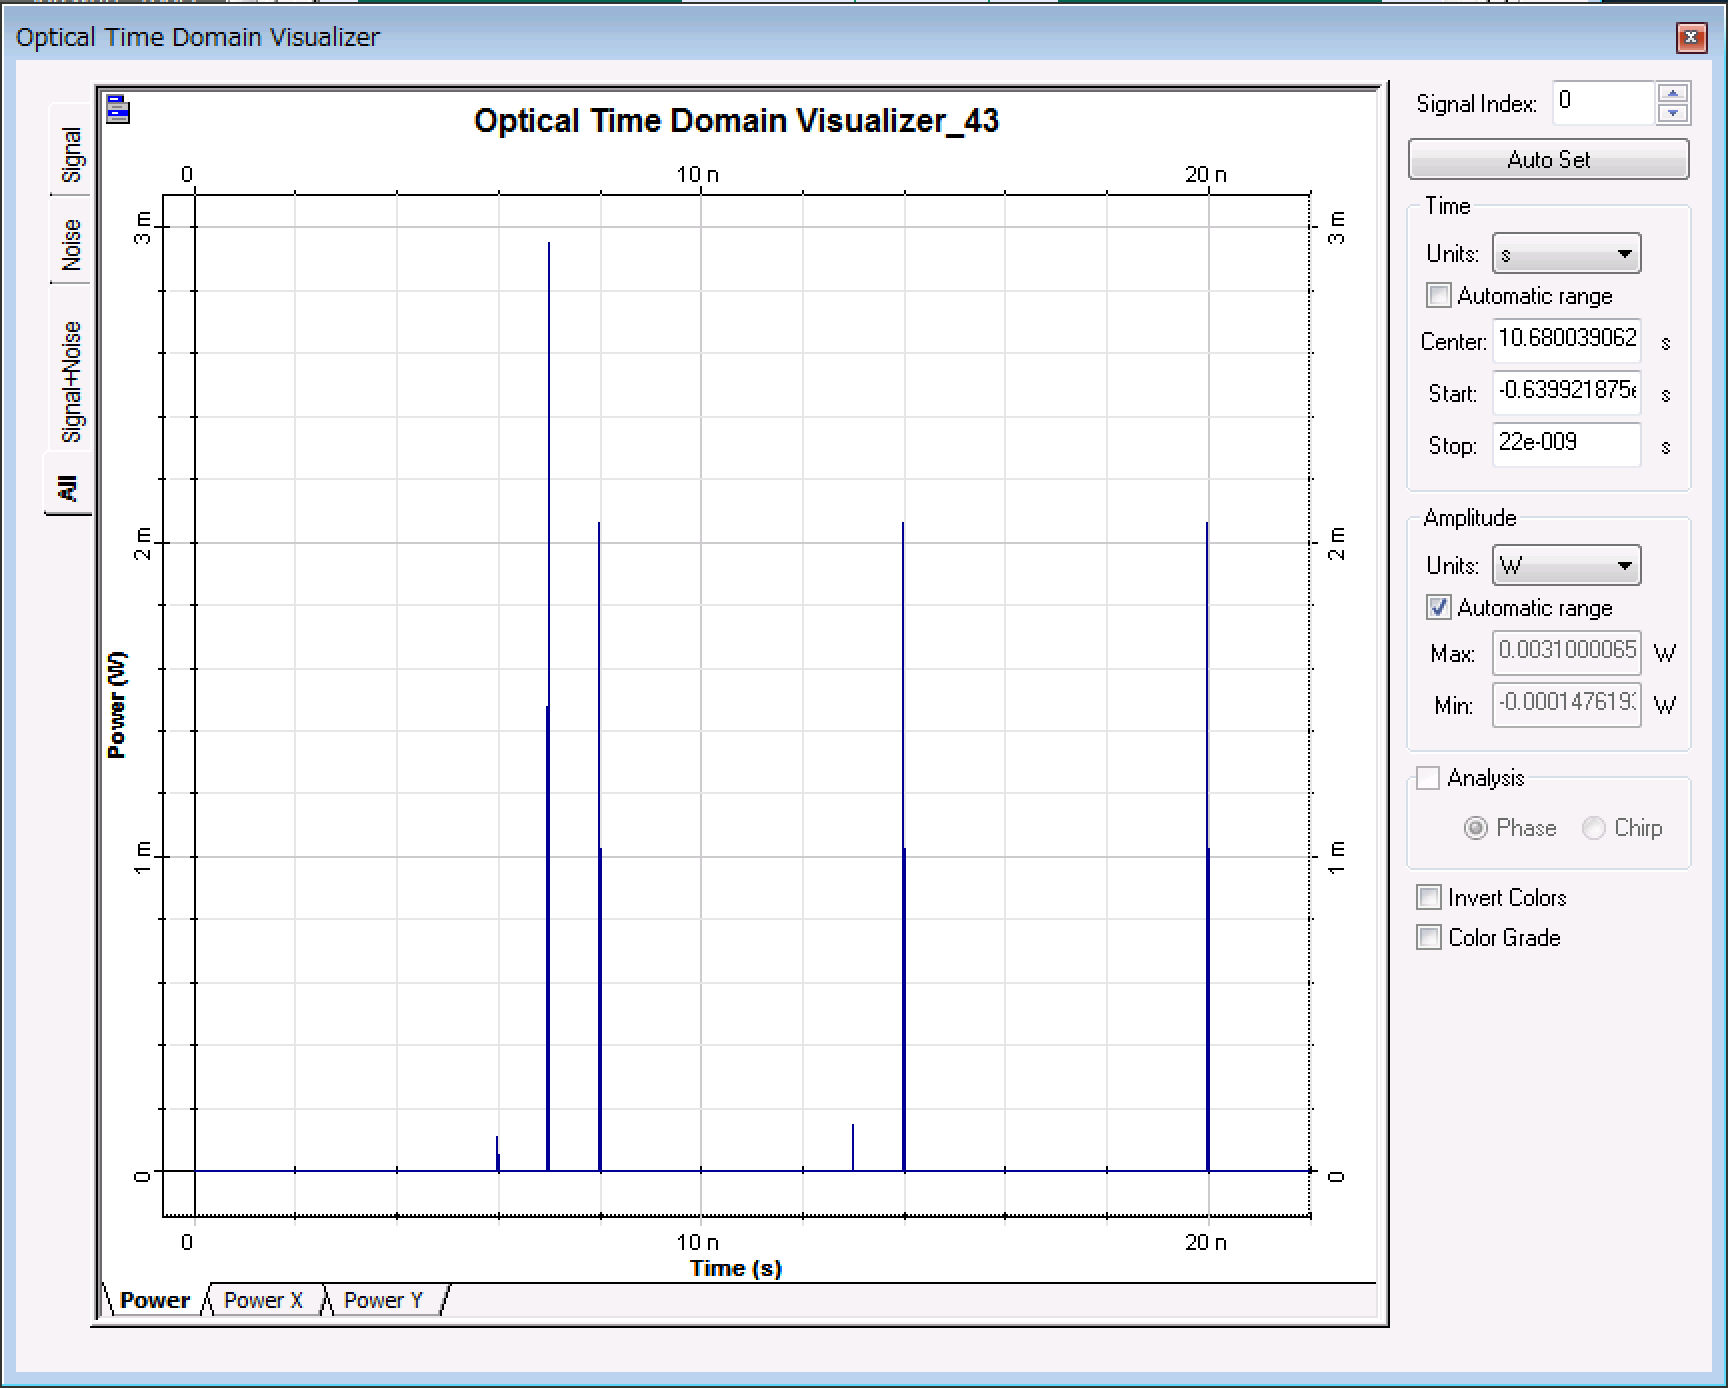
\includegraphics[keepaspectratio,scale=0.5]{fig/4/test_out.png}
\label{test_out}}
\caption{Optisystemによる機能検証結果}
\label{fig:test}
\end{center}
\end{figure}
今回のシミュレーションでは光遅延素子で発生する遅延時間が1nsと設定した.
また配列が一部一致の場合,取りうるスイッチ状態は図\ref{fig:test_swich_b}
だけではない.
今回のシミュレーションでは機能検証上の一例として図\ref{fig:test_swich_b}
の状態を取り扱う.

図\ref{fig:test_swich}のそれぞれの状態において,
出力から最初に観測される信号のタイミングは
入力からns後,ns後,ns後になると想定している.
図\ref{fig:test}のnsnsの区間は図\ref{fig:test_swich_a}の状態,
nsnsの区間は図\ref{fig:test_swich_b}の状態,
nsnsの区間は図\ref{fig:test_swich_c}の状態である.
図\ref{fig:test}を見ると,想定した動作をしているのが確認できる.

\section{評価}

